\documentclass{article}    
\usepackage[utf8]{inputenc}    
    
\title{Épisode 4}    
\author{Jean-Baptiste Bertrand}    
\date{\today}    
    
\setlength{\parskip}{1em}    
    
\usepackage{physics}    
\usepackage{graphicx}    
\usepackage{svg}    
\usepackage[utf8]{inputenc}    
\usepackage[T1]{fontenc}    
\usepackage[french]{babel}    
\usepackage{fancyhdr}    
\usepackage[total={19cm, 22cm}]{geometry}    
\usepackage{enumerate}    
\usepackage{enumitem}    
\usepackage{stmaryrd}    
\usepackage{mathtools,slashed}
%\usepackage{mathtools}
\usepackage{cancel}
    
\usepackage{pdfpages}
%packages pour faire des math    
%\usepackage{cancel} % hum... pas sur que je vais le garder mais rester que des fois c'est quand même sympatique...
\usepackage{amsmath, amsfonts, amsthm, amssymb}    
\usepackage{esint}  
\usepackage{dsfont}

\usepackage{import}
\usepackage{pdfpages}
\usepackage{transparent}
\usepackage{xcolor}
\usepackage{tcolorbox}

\usepackage{mathrsfs}
\usepackage{tensor}

\usepackage{tikz}
\usetikzlibrary{quantikz}
\usepackage{ upgreek }

\newcommand{\incfig}[2][1]{%
    \def\svgwidth{#1\columnwidth}
    \import{./figures/}{#2.pdf_tex}
}

\newcommand{\cols}[1]{
\begin{pmatrix}
	#1
\end{pmatrix}
}

\newcommand{\avg}[1]{\left\langle #1 \right\rangle}
\newcommand{\lambdabar}{{\mkern0.75mu\mathchar '26\mkern -9.75mu\lambda}}

\pdfsuppresswarningpagegroup=1

\usepackage[final]{pdfpages}

\begin{document}
2022-34-29

\section*{Retour sur les spineurs} 


On peut montrer que $\psi ^{\dagger} \vec{\sigma} X$ est un vecteur.

Pour se faire on va transformer que la quantité $\psi ^{\dagger} \vec\sigma \cdot \vec A$, qui devrait être un scalaire, par une rotation. 

$$\to \psi ^{\dagger} R ^{\dagger} \vec \sigma \vec \sigma R X \cdot \mathcal{R} \vec A $$ 

$$\psi ^{\dagger} \simga_i X A_i = \psi ^{\dagger} R ^{\dagger} \sigma_i R X \mathcal{R}_{ij} A_j  = \psi ^{\dagger} R^{\dagger}\sigma_j R X \mathcal{R}_{ji} A_i $$ 

$$\psi ^{\dagger} \sigma_i X = \psi ^{\dagger} R ^{\dagger} \sigma_j R X \mathcal{R}_{ji} $$ 

$$R\sigma_i R ^{\dagger} = \mathcal{R}_{ji} \sigma_j $$ 

$$\boxed{R^{\dagger} \sigma_i R = \mathcal{R} _{ij} \simga_j }$$ 


On représente un vecteur à trois composante par un matrice

$$\vb{r} = \mqty(x & y &z)$$ 

$$X = \vec{r} \cdot \vec\sigma = \mqty[z & x-iy\\x+iy &- z ]$$ 

$$\tr X = 0 \qquad \det X = - \vb{r}^2$$ 

alors


$$X' = R \sigma_i R ^{\dagger} x_i =  RX R ^{\dagger}$$ 


On fait maintenant la même chose pour des 4-vecteurs.


$$X(x)= \mqty[x^{0}-x^{3} & -x^{1}+ix^{2}\\ -x^{1}-ix^{2} & x^{0}+ x^{3}] = x^{0}\mathds{1} - x^{3}\sigma_3 -x^{1}\sigma_1 -\x^{2}\sigma^{3} = x_{\mu} \sigma^{\mu}$$ 

$$\det X = x_{\mu} x^{\mu}$$ 

$$\det X = \det X'\qquad X = N^{\dagger}X'N \qquad \det N =1$$ 

$$\det X = \det X'$$ 

On a deux contraintes sur 8 degrés de liberté (4 degrés complex) et on impose deux contraintes sur les determinant. On a donc 6 degrés de liberté qui correspondent à ceux des trasformation de Lorentz. 



\begin{align*}
	x^{\prime\nu} &= \Lambda_{\nu}^{\mu}x^{\nu}\\
	x'_\mu &= \Lambda_{\mu}^{\nu}x_{\nu} = (\Lambda ^{-1})_\mu^{\nu}x_{\nu} \\
	X' = x'_\mu \sigma^{\mu}=  \Lambda_{\mu}^{\nu}x_{\nu} \sigma_{\mu}\\
	\dotsb
\end{align*}

$$\boxed{N^{\dagger}\sigma^{\mu}N = \Lambda_{\nu}^{\mu}\sigma^\nu}$$ 


C'est vrai pour un définiton de type 1, pour le type 2 (avec les +) on aurait $$M^{\dagger}\tilde \sigma^{\mu}M = \Lambda_{\nu}^{\mu}\sigma^{\nu}$$ 

\hrule


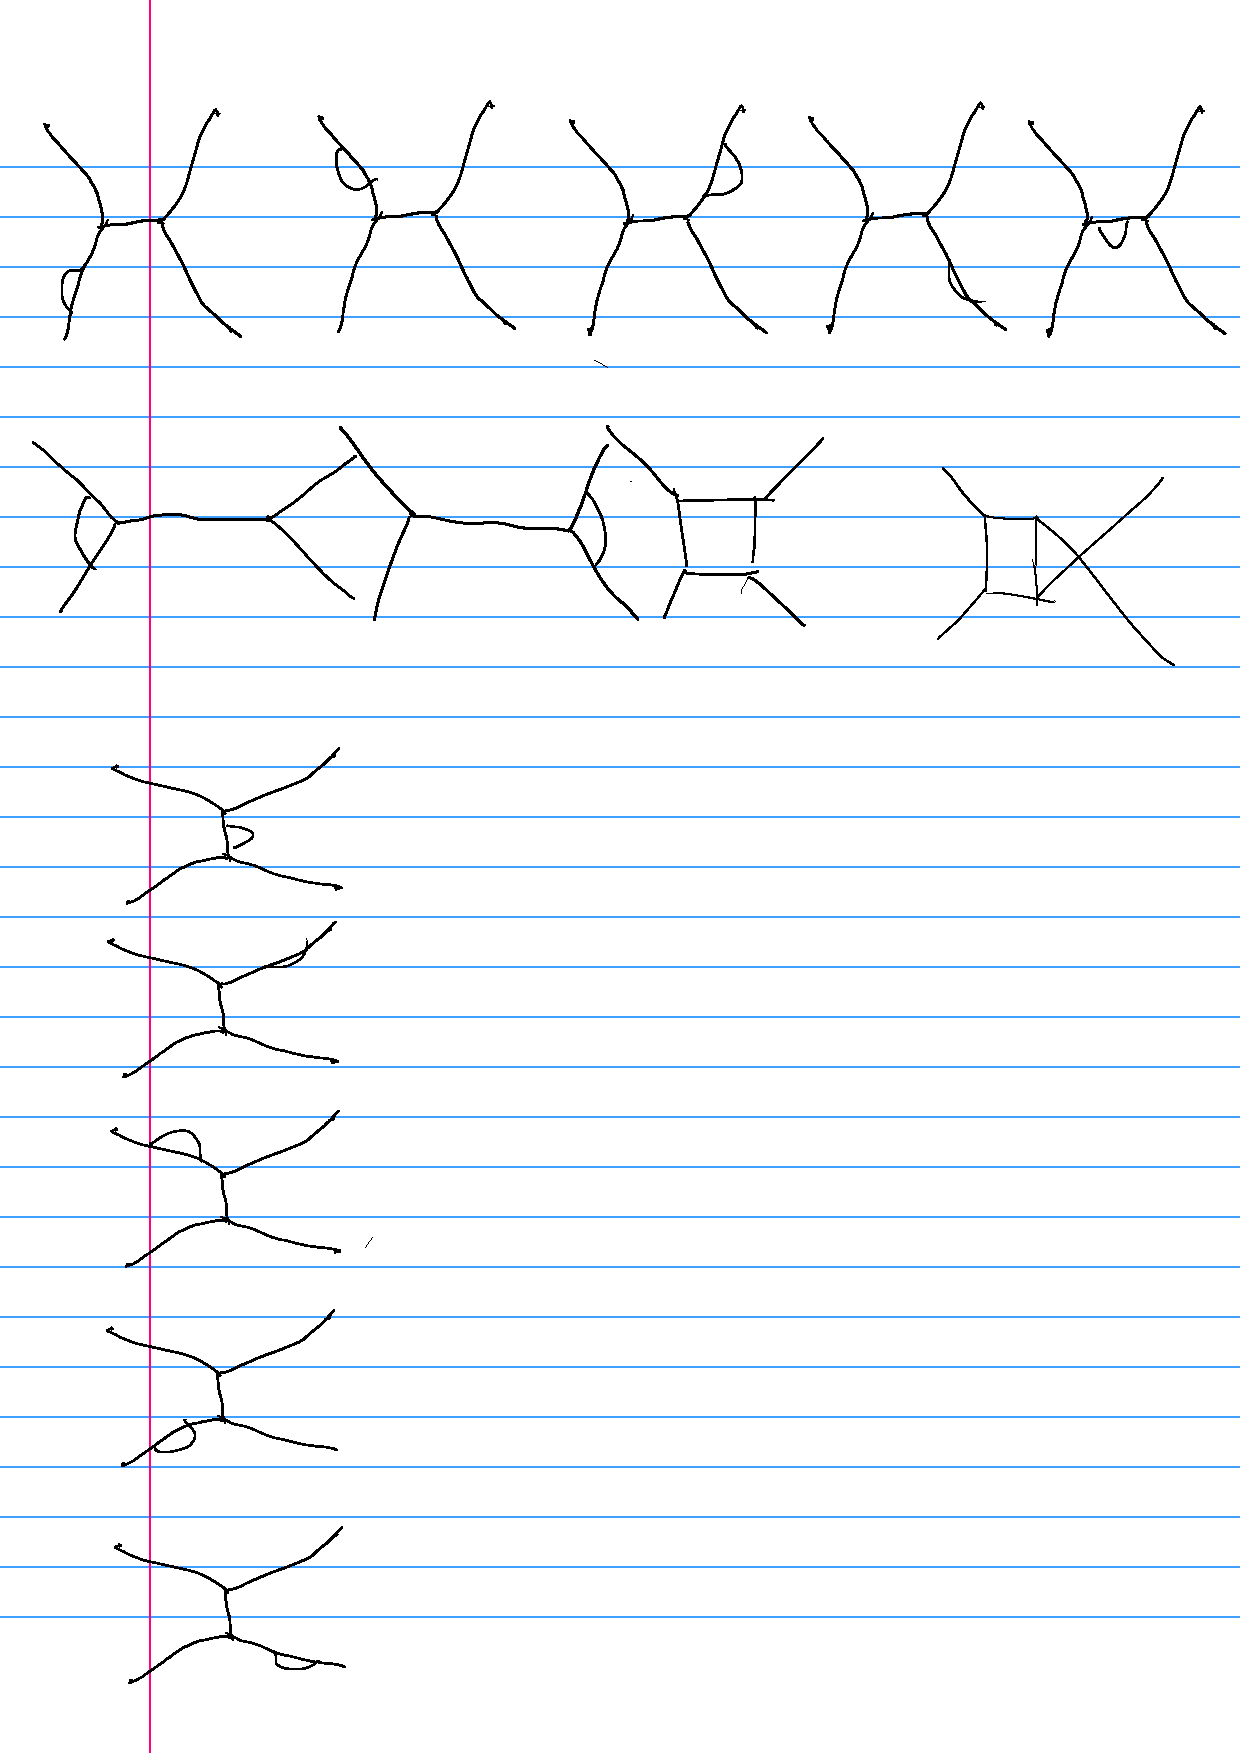
\includepdf[pages=-]{feynman.pdf}

\section*{Théorie en $\phi^{4}$ }

$$\mathscr{L} = \frac{1}{2} \del_{mu} \phi \del^{\mu}\phi - \frac{1}{2} m^{2}\phi^{2} - \frac{g}{4!} \phi^4$$ 


Le premier ordre en énérgie ne s'annule pas, c'est donc plus simple

$$H_1 = \frac{g}{4!}  \int \dd ^3 vr \phi^{4} \left( a + a^{\dagger} \right)\left( a + a^{\dagger} \right)\left( a + a^{\dagger} \right)\left( a + a^{\dagger} \right)  $$ 
 

$$M_{fi}  = \mel{f}{H}{i}= g$$ 

\end{document}
